\documentclass[12pt,letterpaper,noanswers]{exam}
\usepackage[usenames,dvipsnames,svgnames,table]{xcolor}
\usepackage[margin=0.9in]{geometry}
\renewcommand{\familydefault}{\sfdefault}
\usepackage{multicol}
\usepackage{wrapfig}
\pagestyle{head}
\definecolor{c03}{HTML}{FFDDDD}
\header{AM 22b Class 27}{}{Apr 5: Flux and divergence, p. \thepage}
\runningheadrule
\headrule
\usepackage{graphicx} % more modern
\usepackage{amsmath} 
\usepackage{amssymb} 
\usepackage{hyperref}
\usepackage{tcolorbox}
\usepackage[utf8]{inputenc}
\usepackage{diagbox}
\usepackage{graphicx} 
\usepackage{enumitem}
\usepackage{tikz}
\tikzstyle{startstop} = [rectangle, rounded corners, minimum width=3cm, minimum height=1cm,text centered, draw=black]

\tikzstyle{process} = [rectangle, minimum width=3cm, minimum height=1cm, text centered, draw=black, fill=gray!20]
\tikzstyle{decision} = [ellipse, minimum width=3cm, minimum height=0.5cm, text centered, draw=black, fill=white!30]
\tikzstyle{arrow} = [thick,->,>=stealth]
\usetikzlibrary{shapes.geometric, arrows}
\pagenumbering{arabic}

\usepackage[numbered,autolinebreaks,useliterate]{mcode}

\newcommand{\mb}[1]{\underline{#1}}

\begin{document}
 \pdfpageheight 11in 
  \pdfpagewidth 8.5in




% I need to review the torus trajectories...

\begin{itemize}
% \item There is a pre-class assignment (20 minutes of videos + a few WeBWorK exercises) due at 10am this Monday.  It is available on Canvas.
\itemsep0em
\item There is a skill check today (C25, 26).
\item There will be a pre-class assignment for Monday Apr 12th.
\item Problem set 08 is due on Thursday April 8th.
\end{itemize}

\hrule
\vspace{0.2cm}

% partial derivatives, gradient
% local linearity, differential, directional deriv
% 2nd order partials + equations with partials

\noindent\textbf{Big picture}

We are computing flux integrals, where we calculate how much a vector field pushes across a curve or surface.  For the flux out of a closed surface (or curve) we will have a theorem similar to Green's theorem, where we will integrate the flux density (the divergence) over a region to find the flux out the boundary of the region.

\vspace{0.2cm}
\hrule
\vspace{0.2cm}

\noindent\textbf{Skill Check Practice}
\begin{questions}
\item Set up an integral to compute the flux of $\mb F = \cos y\mb i + z\mb j + \mb k$ through $S$ where $S$ is oriented upward and is the part of the surface $z = x^2+2y$ above the region $0\leq x\leq 2, 0\leq y\leq 1$.
\end{questions}

\vspace{0.2cm}
\hrule
\vspace{0.2cm}

\noindent\textbf{Skill Check Practice Solution}

$f(x,y) = x^2+2y$ so $f_x = 2x$, $f_y = 2$.  The vector $\mb u = \langle -f_x, -f_y, 1\rangle$ is normal to $f$ and points upwards.  It is $\mb u = \langle -2x, -2, 1\rangle$.

The component of $\mb F$ pushing upwards through $z = f(x,y)$ is $\mb F \cdot \dfrac{\mb u}{\Vert \mb u \Vert}$.  On the surface, $\mb F = \cos y\mb i + (x^2+2y)\mb j + \mb k$, so $\mb F\cdot \mb u = -2x\cos y -2(x^2+2y) + 1$



We have 
\begin{align*}
\int_S \mb F\cdot d\mb A &= \int_S \mb F \cdot \dfrac{\mb u}{\Vert \mb u\Vert}dS \\
&= \int_R \mb F \cdot \dfrac{\mb u}{\Vert \mb u\Vert} \Vert\mb u\Vert dA \\
&= \int_R \mb F \cdot \mb u\ dA \text{ (you can jump straight to this expression)}\\
&= \int_0^1 \int_0^2 (-2x\cos y -2(x^2+2y) + 1) dx dy
\end{align*}

Recall that $S$ is the original surface (in $3$-space) and $R$ is its projection/shadow in the $xy$-plane.  In this problem, $R$ was specified in the problem statement. $dS$ is a tiny piece of $S$ while $dA$ is a tiny piece of $R$.  (But $d\mb A$ and $d\mb S$ are each used to refer to the area vector associated with a tiny piece of $S$).

\vspace{0.2cm}
\hrule
\vspace{0.2cm}

\noindent\textbf{Teams}
\begin{multicols}{2}

1.  student names
\end{multicols}

\vspace{0.2cm}
\hrule
\vspace{0.2cm}
\eject
\vspace{0.2cm}
\hrule
\vspace{0.2cm}
\noindent\textbf{Computing a surface integral: finding a flux} \S 19.2
\begin{tcolorbox}
\begin{itemize}
\itemsep0em
    \item To set up a flux integral $\displaystyle \int_S \mb F\cdot d\mb A = \int_S \mb F \cdot \mb n\ dS$ where $\mb n$ is a unit vector normal to the surface and $dS$ is a piece of the surface:
    \item When $S$ is a part of the graph $z = f(x,y)$ oriented upward, $\displaystyle d\mb A = \mb n dS = \frac{\langle -f_x, -f_y,1\rangle}{\sqrt{f_x^2+f_y^2+1}} dS = \frac{\langle -f_x, -f_y,1\rangle}{\sqrt{f_x^2+f_y^2+1}}\sqrt{f_x^2+f_y^2+1} dA = \langle -f_x, -f_y,1\rangle dA$, where $dA$ is a piece of $R$, the projection of $S$ onto the $xy$-plane.  \item When $S$ is a part of the graph $z = f(x,y)$ oriented upward, $\displaystyle \int_S \mb F\cdot d\mb A = \int_R \mb F(x,y,f(x,y))\cdot \langle -f_x, -f_y, 1\rangle dA$.  \emph{Notice that the first integral is over $S$ and the second is over $R$.}
    \item We will look at other cases (where $S$ cannot be written as a part of a graph) on a different day.
\end{itemize}


\end{tcolorbox}
\noindent\textbf{Example (setting up a flux integral through a graph)}.

Compute the flux of $\mb F = z\mb k$ through $S$ where $S$ is the portion of the plane $x+y+z=1$ in the first octant, oriented upward.

\begin{enumerate}
\itemsep3em
    \item Find $f(x,y)$ so that $z = f(x,y)$ (making $S$ a piece of the graph $z = f(x,y)$).  %Rewrite $x+y+z = 1$ as $z = 1-x-y$, so $z=f(x,y)$ with $f(x,y) = 1-x-y$.
    \item Find $d\mb A = \langle -f_x, -f_y, 1\rangle dA$ for this surface. %Find $\mb n = \langle -f_x,-f_y,1\rangle$.  $\mb n = \langle 1, 1, 1\rangle$ for this surface.
    \item Compute $\mb F(x,y,z)\cdot \langle -f_x, -f_y, 1\rangle$ (this is sometimes $0$ or constant so is worth doing first).  %We have $\mb F\cdot \mb n = z.$
    \item Find $\mb F(x,y,f(x,y))\cdot \langle -f_x, -f_y, 1\rangle$, so that $\mb F$ is being computed on the surface $S$. %, so sub $f(x,y)$ in place of $z$.  We find $\mb F(x,y,f(x,y))\cdot \mb n = 1-x-y$.
    \item Identify the region $R$ in the $xy$-plane corresponding to $S$.  %Here, $x,y,z\geq 0$.  When $z = 0$, $x+y = 1$ so in the first octant the plane is above a triangle bounded by $x =0, y=0, x+y=1$.
    \item Set up the integral $\displaystyle \int_R \mb F\cdot \mb n dA$.  %In this case we have $\displaystyle\int_0^1\int_0^{1-x}(1-x-y)dydx.$
    \vspace{1in}
\end{enumerate}

\noindent\textbf{Example (setting up a flux integral through a graph)}.

Set up an integral to compute the flux of $\mb F$ through $S$ where $\mb F = \ln(x^2)\mb i + e^x\mb j + \cos(1-z)\mb k$ and $S$ is the part of the surface $z = -y+1$ above the square $0\leq x\leq 1$, $0\leq y\leq 3$, oriented downward.


\vspace{2in}


\vspace{0.2cm}
\hrule
\vspace{0.2cm}
\noindent\textbf{Flux density (divergence) for 2D vector fields} \S 19.3, \S 18.4
\begin{tcolorbox}
\begin{itemize}
\itemsep0em
    \item Green's theorem related the circulation around the boundary to a very local measure of the rotation of the vector field at each point within a region: have $\oint_C \mb F\cdot \mb T ds = \int_R Q_x - P_y dA$, so $\oint_C Pdx + Qdy = \int_R (Q_x - P_y) dA$.
    \item Identifying the flux outward through a closed curve is asking how much the vector field, in net, pushes out of the region of interest.  Imagine the vector field transporting particles.  When there is a net outward flux, the particles must be spreading out (diverging) somewhere within the enclosed region.  When there is a net inward flux, the particles must be converging somewhere within the enclosed region.
    \item The \textbf{divergence} is a measure of the local spread of an infinitesimal region under the action of the vector field.
    \item Consider a vector field $\mb F = \langle P,Q,R\rangle$.  $\frac{\partial P}{\partial x}$ measures whether the horizontal component of the vectors in the field is lengthening as $x$ increases (positive) or shrinking as $x$ increases (negative).  This is a measure of whether the horizontal component of the vector field is driving divergence (positive) or convergence (negative).
    \item The \textbf{divergence} of a vector field $\mb F = \langle P,Q,R\rangle$ is given by $\text{div }\mb F = \frac{\partial P}{\partial x}+\frac{\partial Q}{\partial y}+\frac{\partial R}{\partial z}$.  Thinking of the operator $\nabla$ as $\nabla = \langle \frac{\partial }{\partial x},\frac{\partial}{\partial y},\frac{\partial}{\partial z}\rangle$, we can write $\text{div }\mb F = \nabla \cdot \mb F$.
    %\item Let $\displaystyle\mb F = M\mb i + N\mb j$.  $\oint_C \mb F \cdot \mb n ds = \oint_C \mb F \cdot \langle dy, -dx\rangle$.  Rearrange and use Green's theorem to find a flux form of Green's theorem: $\displaystyle\oint_C \mb F \cdot \mb n ds=\oint_C Mdy-Ndx = \oint_C \langle -N, M\rangle \cdot \mb T ds = \int_R (M_x + N_y) dA$.
\end{itemize}
\end{tcolorbox}
\noindent\textbf{Example (traffic on a highway)}.  Consider the traffic on a highway going in a single direction.  At each point on the road, cars move at velocity $M(x)\vec i$ when they reach that point.  We can think of a vector field $\mb v(x) = M(x)\mb i$, defined along the $x$-axis.  

If traffic is steadily slowing down as we move in the positive $x$ direction, are the cars converging together or diverging apart?  What is the sign of $\text{div }\mb v?$


\vspace{1in}

\noindent\textbf{Example (going to class)}.  Vector fields can be time dependent.  Think of a vector field describing the flow of students in space.  Just before class starts, students flow into a classroom.  Just after it ends, they flow out.  In which case will the divergence necessarily be positive at some locations in the classroom?  In which case will it necessarily be negative?

\vspace{1in}

\noindent\textbf{Example (vector fields with constant divergence)}

Each of the following four vector fields has constant divergence everywhere in space.  Identify whether the divergence is positive, negative, or zero.  \emph{The left, center, and right columns show the positions of 25 particles that are being moved under the action of the vector field.  The left column is the earliest time, the center column is a middle time, and the right column is the most recent time.}
%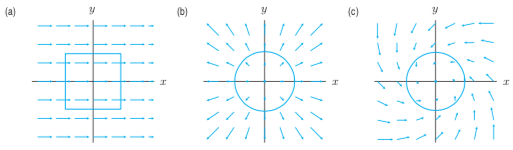
\includegraphics[scale=0.8]{img/C24p1.png}

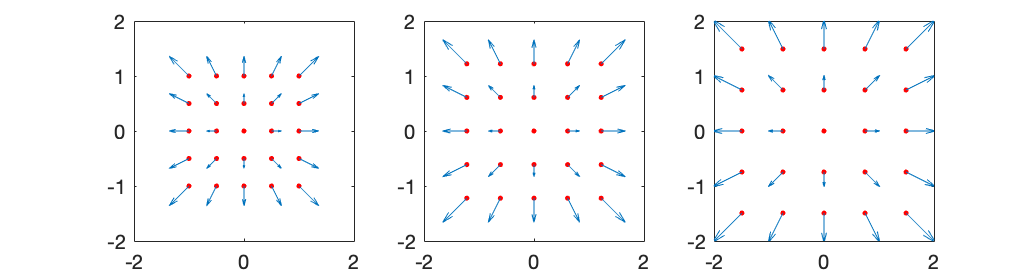
\includegraphics[width=0.9\linewidth]{img/C26p1a.png}

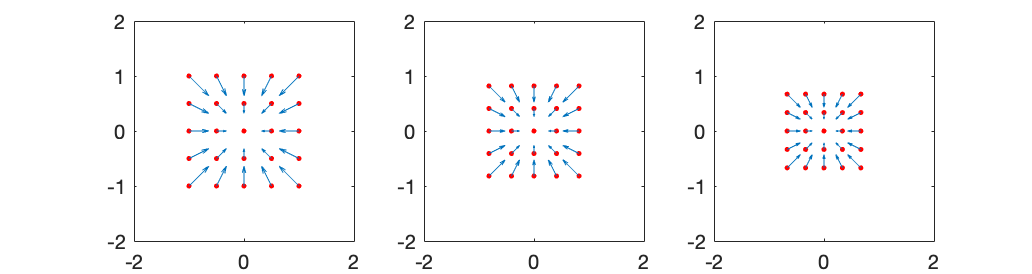
\includegraphics[width=0.9\linewidth]{img/C26p1b.png}

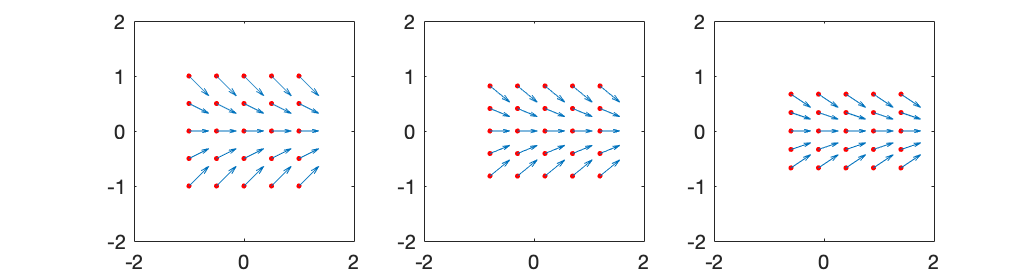
\includegraphics[width=0.9\linewidth]{img/C26p1c.png}

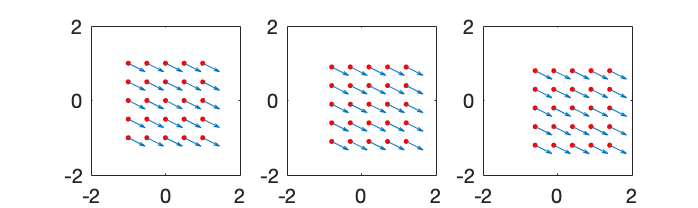
\includegraphics[width=0.9\linewidth]{img/C26p1d.png}




\vspace{0.2cm}
\hrule
\vspace{0.2cm}

\begin{tcolorbox}
\begin{itemize}
\itemsep0em
    \item \textbf{Divergence free} vector fields are sometimes called \emph{solenoidal}.  (Solenoid is a word associated with a particular kind of electromagnet).  The magnetic field (a vector field from physics) is divergence free.
    \item Divergence free vector fields are sometimes called \textbf{incompressible}.  This term is associated with fluid dynamics and is used for fluids (like water) that are modeled as not stretching or compressing parcels of the fluid while they flow under the action of the vector field.
    \item Divergence is sometimes described as the extent to which a vector field behaves like a \textbf{source} at a given point (positive divergence), or like a \textbf{sink} (negative divergence).
\end{itemize}
\end{tcolorbox}

\noindent\textbf{Example (computing divergence)}
Compute the divergence for the following vector fields.
\begin{enumerate}
\itemsep3em
    \item $-y\mb i + x\mb j$
    \item $3x^2\mb i - \sin(xz)(\mb i + \mb k)$
    \item $\mb r - \mb a$ for $\mb a$ a constant vector field (and $\mb r = \langle x,y,z\rangle$.
    \item $\mb a\times \mb r$ for $\mb a$ a constant vector field
    \vspace{1.3in}
\end{enumerate}






\end{document}